\documentclass[twocolumn,english,pra,aps,superscriptaddress,floatfix]{revtex4-1}

\usepackage{amsthm}
\usepackage{amsmath}
\usepackage{graphicx}
\usepackage{amssymb}
%\usepackage{esint}
\usepackage{bm}
\usepackage{latexsym}

\makeatletter
%%%%%%%%%%%%%%%%%%%%%%%%%%%%%% Textclass specific LaTeX commands.
\@ifundefined{textcolor}{}
{%
 \definecolor{BLACK}{gray}{0}
 \definecolor{WHITE}{gray}{1}
 \definecolor{RED}{rgb}{1,0,0}
 \definecolor{GREEN}{rgb}{0,1,0}
 \definecolor{BLUE}{rgb}{0,0,1}
 \definecolor{CYAN}{cmyk}{1,0,0,0}
 \definecolor{MAGENTA}{cmyk}{0,1,0,0}
 \definecolor{YELLOW}{cmyk}{0,0,1,0}
 }

%%%%%%%%%%%%%%%%%%%%%%%%%%%%%% User specified LaTeX commands.
%\numberwithin{equation}{section}

\makeatother

\usepackage{babel}

\begin{document}



\author{N. Miladinovic}
\affiliation{Department of Physics and Astronomy, McMaster University, 1280 Main
St.\ W., Hamilton, ON, L8S 4M1, Canada} 
\author{D.\ H.\ J.\ O'Dell}
\affiliation{Department of Physics and Astronomy, McMaster University, 1280 Main
St.\ W., Hamilton, ON, L8S 4M1, Canada}

\title{Electromagnetic Momenta in a Double Cavity System}

\begin{abstract}
\label{sec:abstract}
We examine the electromagnetic momentum inside a double cavity system in which we allow the difference in cavity lengths to vary.  We show that the dichotomy between the Abraham photon momentum $p_A= p_{0} n_{r}$ and the Minkowski photon momentum $p_M=\frac{p_{0}}{n_{r}}$ may be interpreted as an ambiguity in the partitioning of energy inside the cavity.  Here $p_0$ is the free space momentum of the photon in the cavity, and $n_{r}$ is the refractive index due to the presence of the dielectric slab. The model may be extended to a single atom in a cavity and we show how experimental agreement with both representations may arise. 
\end{abstract}

\pacs{42.50.Ex, 42.50.Pq, 42.60.Da, 42.82.Et, 03.67.Lx}

\maketitle

\section{Introduction}
\label{sec:intro}

There has been a recent resurgence of interest in understanding the electromagnetic momentum density in a dielectric medium \cite{barnett,chiao,mansuripur,ketterle,feng,hinds,loudon}.  Two different forms of the momentum density were given by Minkowski and Abraham.  Minkowski argued that the density be of the form $P_M=D\times B$, while Abraham held that $P_A=\frac{1}{c^2}E\times H$.  For single photons these momenta are given by $p_M= p_{0} n_{r}$ and $p_A=\frac{p_{0}}{n_{r}}$ respectively, where $p_0=\hbar k$ is the momentum in free space . In this paper we consider an electromagnetic field in a cavity interacting with a dielectric slab. The model is solved analytically by making use of a simple $\delta$-function approximation for the central dielectric slab. 
This paper is organized as follows. In Section \ref{sec:deltafunctionmodel} we introduce a simple model for the spatial dependence of the dielectric permittivity function inside a double cavity. This model treats the central mirror as a Dirac $\delta$-function which facilitates analytic calculations. In Section \ref{sec:AnalyticExpressions} we find the global static solutions (normal modes) of Maxwell's wave equation subject to this dielectric function.  From here we are able to extract the refractive index of the cavity-slab system. In Section \ref{sec:force} we determine the optical force on the dielectric slab and wrestle with an ambiguity in system energy which crops up. In Section \ref{sec:Energy} we use the work-energy theorem to determine the form of the energy-momentum density. Conclusions are drawn in Section \ref{sec:conclusion}.




\section{$\delta$-function dielectric model}
\label{sec:deltafunctionmodel}



Consider a double cavity formed from two end mirrors plus a common mirror located between them, as shown Figure \ref{fig:cavitysetup}.  

%***************************figure**********************
\begin{figure}
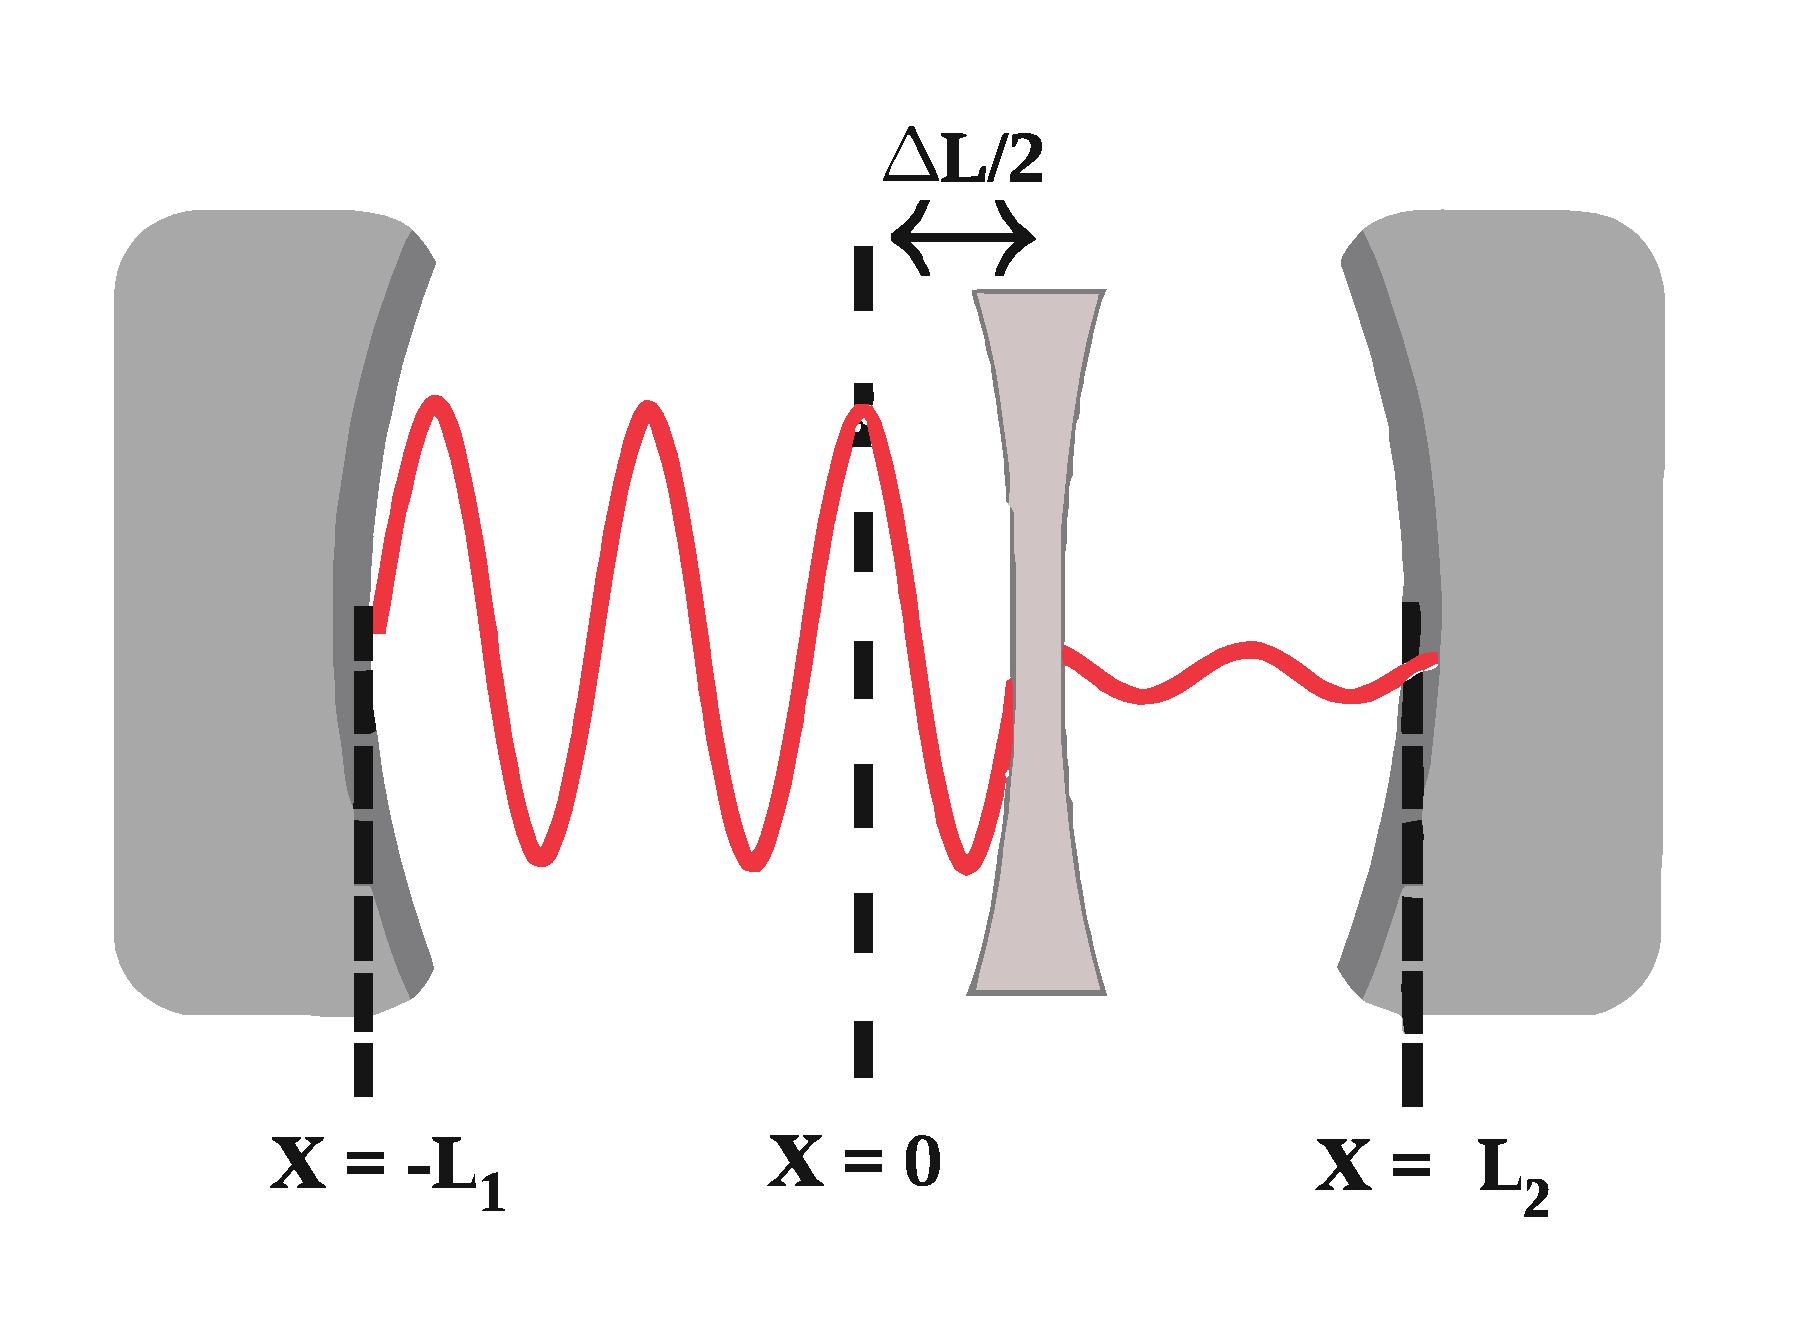
\includegraphics[width=1\columnwidth]{CavitySetupNew.pdf}
\caption{Double cavity setup consisting
of two perfectly reflecting mirrors, along with a partially transmissive common central mirror. $\Delta L \equiv L_{1}-L_{2}$ is the difference in length between the two cavities.}
\label{fig:cavitysetup}
\end{figure}
%*********************************************************

A simple theoretical model describing a double cavity has been given in a classic paper by 
Lang, Scully and Lamb \cite{lang73}. For the purposes of solving Maxwell's wave equation in the double cavity, they treated the end mirrors as perfect reflectors and the central mirror as a thin slab of dielectric material which is modelled by a Dirac $\delta$-function spatial profile. The double cavity model is thereby encoded in a dielectric permittivity function of the form
 \begin{equation}
\varepsilon(x)=\begin{cases}
\varepsilon_{0}(1+\frac{a}{\varepsilon_{0}} \delta(x)) & -L_{1}<x<L_{2}\\
\infty & \mbox{elsewhere}\end{cases}
\label{perm}
\end{equation}
where $x=-L_{1}$, and $x=L_{2}$ are the positions of the end mirrors. $a$ is a parameter which determines the reflectivity of the common mirror.  We have purposely written it in this suggestive manner in anticipation of the findings in Appendix A. The total length of the double cavity is $L \equiv L_{1}+L_{2}$, and we also define the difference between the lengths of the two cavities to be $\Delta L \equiv L_{1}-L_{2}$,  which is also twice the displacement of the common mirror from the center of the whole cavity. 




Maxwell's wave equation for the electric field $\mathcal{E}(x,t)$ in the double cavity is
\begin{equation}
\frac{\partial^{2}\mathcal{E}(x,t)}{\partial x^{2}}-\mu_{0}\varepsilon_{0}(1+\frac{a}{\varepsilon_{0}}\delta(x))\frac{\partial^{2}\mathcal{E}(x,t)}{\partial t^{2}}=0 \ .
\label{maxwell}
\end{equation}
We use this $\delta$-mirror model because its simplicity facilitates analytic results.  


We write the solutions to the Maxwell wave equation as $\mathcal{E}_{m}(x,t)=U_{m}(x) \exp(-i\omega_{m}t)$,  where $\omega_{m}=k_{m}/\sqrt{\varepsilon_{0}\mu_{0}}$ is the angular frequency and $m=1,2,3 \ldots$ is an integer labeling the modes. The dimensionless mode functions $U_{m}(x)$ can be chosen to be orthogonal
in the Sturm-Liouville sense by ensuring that they obey
\begin{equation}
\frac{1}{\varepsilon_{0}}\int_{-L_{1}}^{L_{2}}\varepsilon(x)U_{l}(x)U_{m}(x)dx=0 \quad  l \neq m
\label{normalization}
\end{equation}
Inserting the above form for $\mathcal{E}(x,t)$ into Eq.\ (\ref{maxwell}) gives
\begin{equation}
\frac{\mathrm{d}^{2}U_{m}(x)}{\mathrm{d}x^{2}}+k_{m}^{2}(1+\frac{a}{\varepsilon_{0}}\delta(x))U_{m}(x)=0 \ .
\label{maxwell2}
\end{equation}
Solutions satisfying the boundary conditions $U_{m}(-L_{1})=U_{m}(L_{2})=0$
are given by
\begin{equation}
U_{m}(x)=\begin{cases}
\mathcal{A}_{Lm}\sin \left[k_{m}(x+L_{1})\right]\quad & -L_{1} \leq x\leq0\\
\mathcal{A}_{Rm}\sin \left[k_{m}(x-L_{2})\right]\quad & \,\:\:\:0 \leq x \leq L_{2} \ . \end{cases}
\label{Wavemode}
\end{equation}
Assuming the electric field is continuous across
the $\delta$-mirror, so that $U_{m}(0^{+})=U_{m}(0^{-})$, we can integrate Eq.\ (\ref{maxwell2}) over a vanishingly small interval containing the mirror and thereby find the last boundary condition
$U_{m}^{\prime}(0^{+})-U_{m}^{\prime}(0^{-})=-\frac{a}{\varepsilon_{0}} k_{m}^{2}U_{m}(0)$.



Combining all the boundary conditions one is led to the following equation
for the wave numbers $k_{m}$ of the allowed modes \cite{lang73}
\begin{equation}
\cos(k_{m} \Delta L)-\cos(k_{m} L)=2\varepsilon_{0} \ \frac{\sin k_{m} L}{a k_{m}} \ .
\label{transcendental}
\end{equation}
This transcendental equation can in general only be solved numerically. However, when $a k$ becomes large the sinc function on the right hand side becomes small. The left hand side may then be expanded around its roots and this permits approximate analytic solutions which will be supplied in Section \ref{sec:AnalyticExpressions}.
We refer to the solutions for the wave number in the case of an empty cavity system (i.e when there is no central mirror) as $k_0$.




\section{Analytic Results}
\label{sec:AnalyticExpressions}



The mode amplitudes $\mathcal{A}_{Lm}$ and $\mathcal{A}_{Rm}$ on the two sides of the common mirror are calculated.  From the continuity condition for the field across the mirror we find that   
\begin{equation}
\frac{\mathcal{A}_{Lm}}{\mathcal{A}_{Rm}}=-\frac{\sin(k_{m}L_{2})}{\sin(k_{m}L_{1})} = -\frac{\sin [k_{m} (L-\Delta L)/2]}{\sin[k_{m}(L+\Delta L)/2]} 
\label{A/B} 
\end{equation}

Throughout this paper we make use of results obtained by considering a closed cavity system.  Although not physical, the results approximate an open cavity system in which the end mirrors are much more reflective than the central mirror.   In  Figure \ref{fig:openvsclosed} we compare the amplitude ratio found in Eq.\ (\ref{A/B}) with numerical solutions obtained for an open cavity system.  The end mirrors are assumed to be 10 times more reflective than the central mirror. We see that the field distribution coincides very well with the closed cavity.


%***************************figure**********************
\begin{figure}
%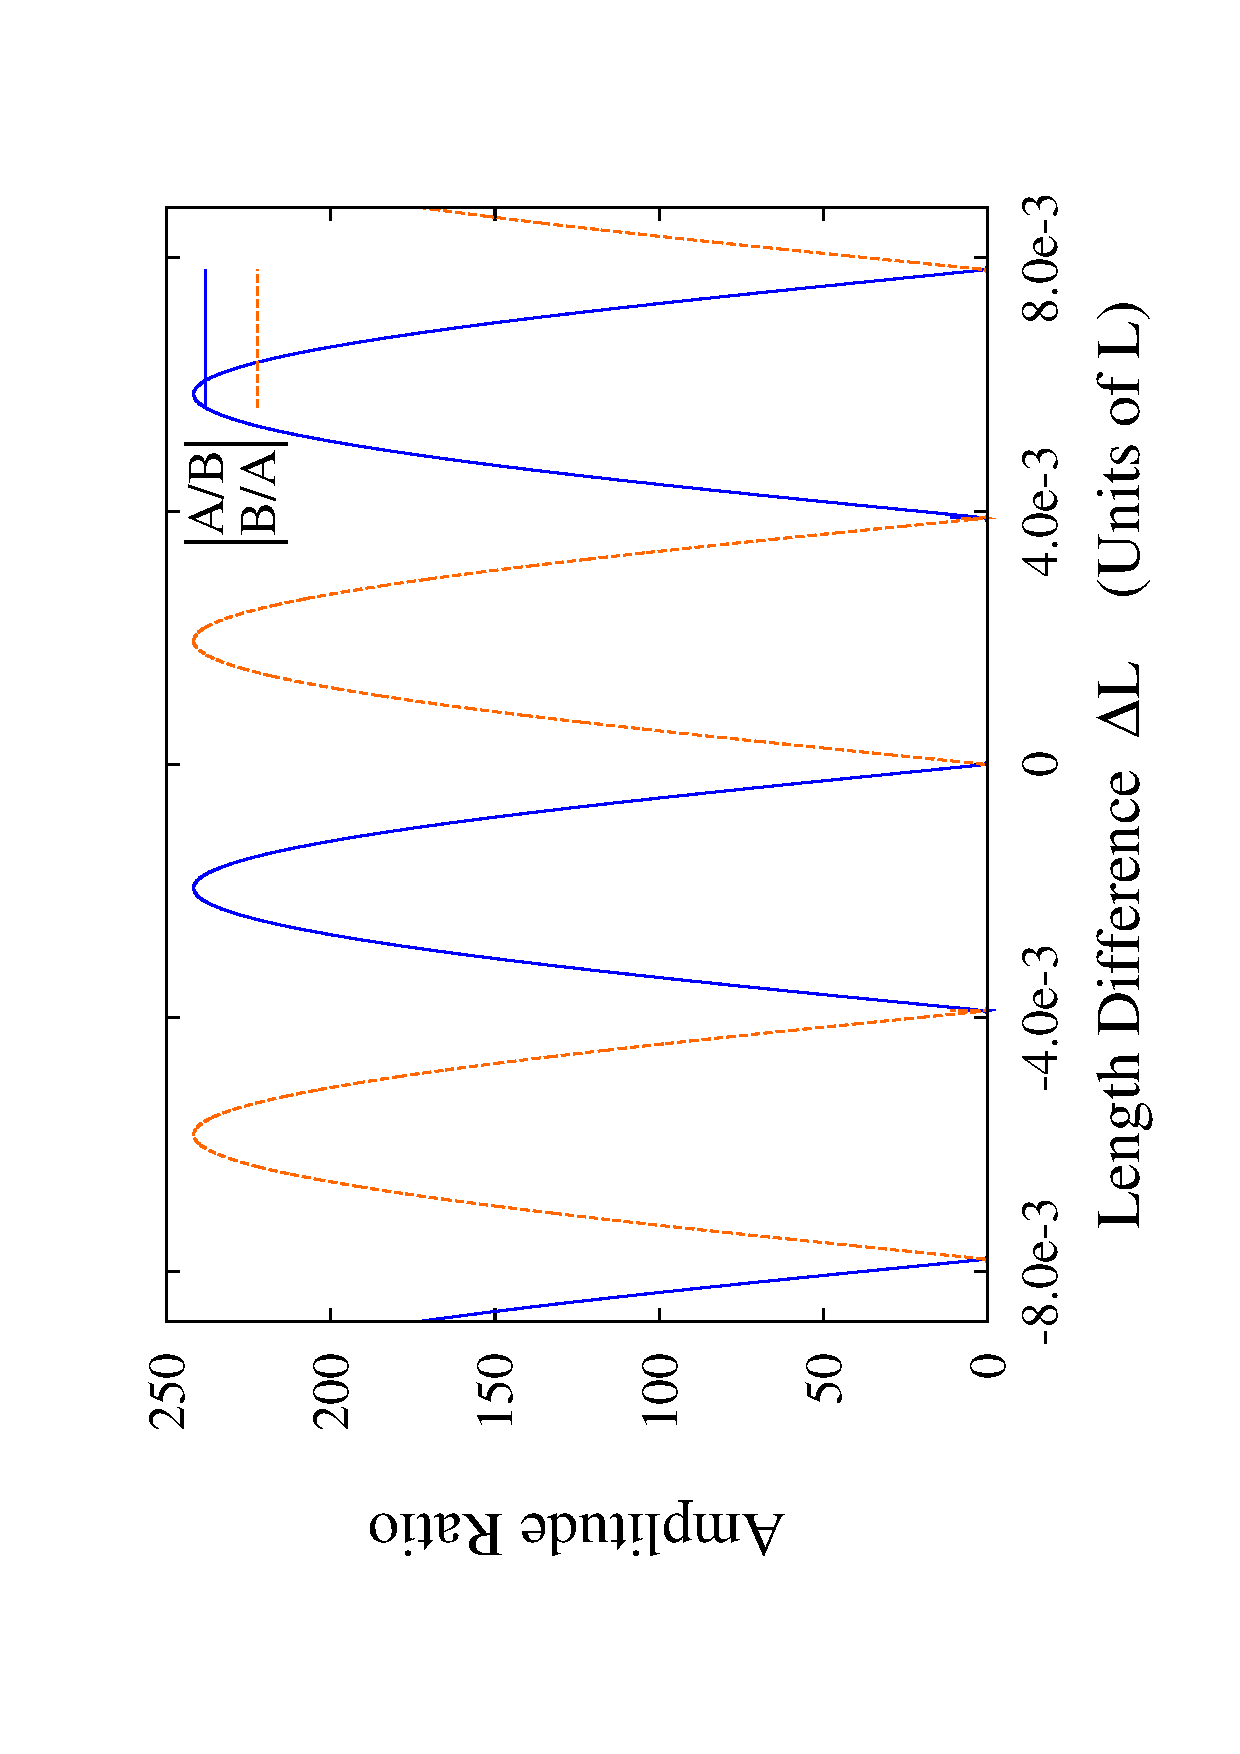
\includegraphics[width=1\columnwidth]{AmplitudeRatio}
\caption{The relative amplitude ratio Eq.\ (\ref{A/B}) is plotted (red) along side numeric solutions solved using Maxwell's equations in an open cavity system (blue).  In the open system, the outer mirrors were set to be 10 times more reflective than the central mirror.}
\label{fig:openvsclosed}
\end{figure}
%*********************************************************

We now turn back to the transcendental equation Eq.\ (\ref{transcendental}) . It is possible to find an analytic solution for the wave number $k_{m}$ when $a$
is very small as it is for a low density atomic cloud. When $a$ is very small, the right side of Eq.\ (\ref{transcendental}) must still
be of order one, therefore $\sin kL$ must be very close to zero. We therefore expand $kL$ about $m\pi$ to first order 

\begin{equation}
\cos(k\triangle L)\pm1=\mp\frac{2\varepsilon_{0}L}{a}\left(\frac{1}{m\pi}\left(x-m\pi\right)\right)
\label{transcendental2}
\end{equation}

Now $\cos(k\Delta L)$ has a $k$ in the argument, however as this doesn't deviate from $m\pi$ much, it is reasonable for small values of $a$
to replace it with $m\pi$ as the cosine function is insensitive to such small perturbations 

\begin{equation}
k_{m}=\pm\frac{a m\pi}{2\varepsilon_{0}L^{2}}\left(\cos(m\pi\frac{\triangle L}{L})\mp1\right)+\frac{m\pi}{L}
\label{wavenumber1}
\end{equation}

Note that the upper signs correspond to odd $m$ and lower signs to
even $m$ respectively.  In Figure \ref{fig:wavenumberapprox} we plot Eq.\ (\ref{wavenumber1}) against the numeric solution for the wave number. 



%***************************figure**********************
\begin{figure}
%\includegraphics[width=0.8\columnwidth]{WavenumberApprox}
\caption{Wavenumber is plotted as a function of central mirror position.  The analytic result Eq.\ (\ref{wavenumber1}) is in blue, and the numeric solution is plotted in red.  In the plot the value of $a$, which controls the strength of the $\delta$-potential, is set at $a=10^{-5}$. }
\label{fig:wavenumberapprox}
\end{figure}
%*********************************************************

We now ask ourselves what the effective refractive index is for the system. For this we rewrite Eq.\ (\ref{wavenumber1}) as
\begin{equation}
k_{m}=\frac{m\pi}{L}\left[\pm\frac{a}{2\varepsilon_{0}L}\left(\cos(m\pi\frac{\triangle L}{L})\mp1\right)+1\right]=k_{0} n_{r}
\label{wavenumber2}
\end{equation}
and we can easily extract the effect refractive index

\begin{equation}
n_{r}=\left[\pm\frac{a}{2\varepsilon_{0}L}\left(\cos(m\pi\frac{\triangle L}{L})\mp1\right)+1\right]
\label{refractiveindex}
\end{equation}

where the upper signs correspond to odd $m$ while lower signs give the result for even $m$.  

\section{The Force on a dielectric material in a cavity}
\label{sec:force}
We turn to the problem of calculating the electromagnetic force on the central mirror, which will allow for a simple calculation of the momentum transfer. We begin by noting that the force $F$ is given by the momentum flux integrated about a gaussian pillbox containing the dielectric slab \cite{domokos08} (see Figure \ref{fig:gaussianpillbox}).  This optical force is the rate at which momentum is being extracted from the electromagnetic field due to the presence of the mirror  \cite{griffiths}.  

%***************************figure**********************
\begin{figure}
\includegraphics[width=1\columnwidth]{GaussianPillbox}
\caption{The force is found by integrating the Maxwell stress tensor around a small pillbox containing the central mirror}
\label{fig:gaussianpillbox}
\end{figure}
%*********************************************************

\begin{equation}
F=\oint_{S}\overleftrightarrow{T}\cdot da-\varepsilon_{0}\mu_{0}\frac{\partial}{\partial t}\int_{V}Sd\tau
\label{stresstensor1}
\end{equation}
where $T$ is the Maxwell stress tensor defined as

\begin{equation}
T_{xx}=\frac{\varepsilon_{0}}{2}\left(\mathcal{E}_{x}^{2}-\mathcal{E}_{y}^{2}-\mathcal{E}_{z}^{2}\right)+\frac{1}{2\mu_{0}}\left(B_{x}^{2}-B_{y}^{2}-B_{z}^{2}\right)
\label{stresstensor2}
\end{equation}


\begin{equation}
T_{xy}=\varepsilon_{0}\left(\mathcal{E}_{x}\mathcal{E}_{y}\right)+\frac{1}{\mu_{0}}\left(B_{x}B_{y}\right)
\label{stresstensor3}
\end{equation}
$S$ in Eq.\ (\ref{stresstensor1}) is the poynting vector, which is zero for a stationary system.  As we are only considering the stationary modes of the system this term drops out.
If we write the modes to the left and to the right of the dielectric
slab respectively as

\begin{equation}
\mathcal{E}_{L}=\mathcal{E}_{1}e^{ikx}+\mathcal{E}_{2}e^{-ikx}
\label{Efieldleft}
\end{equation}


\begin{equation}
\mathcal{E}_{R}=\mathcal{E}_{3}e^{ikx}+\mathcal{E}_{4}e^{-ikx}
\label{EfieldRight}
\end{equation}

We then arrive at the force per unit area $F$ 

\begin{equation}
F=\frac{\varepsilon_{0}}{2}\left(\left|\mathcal{E}_{1}\right|^{2}+\left|\mathcal{E}_{2}\right|^{2}-\left|\mathcal{E}_{3}\right|^{2}-\left|\mathcal{E}_{4}\right|^{2}\right)
\label{force1}
\end{equation}

To proceed we require the amplitudes $\mathcal{E}_{1}$, $\mathcal{E}_{2}$, $\mathcal{E}_{3}$, $\mathcal{E}_{4}$. What we have instead is an analytic solution for the amplitudes
of the two standing waves to the left and to the right of the dielectric slab as is given by Eq.\ (\ref{A/B}).
If we rewrite the standing wave as the composite of two traveling waves moving in opposite direction, then we require $\mathcal{E}_{Lm}=2\mathcal{E}_{1}=2\mathcal{E}_{2}$, and $\mathcal{E}_{Rm}=2\mathcal{E}_{3}=2\mathcal{E}_{4}$.
Plugging this into Eq.\ (\ref{force1}) we obtain

\begin{eqnarray}
F&=&\frac{\varepsilon_{0}}{4}\left(\left|\mathcal{E}_{Lm}\right|^{2}-\left|\mathcal{E}_{Rm}\right|^{2}\right)\nonumber \\ &=&\left(\frac{\varepsilon_{0}}{4}\left|\mathcal{E}_{Rm}\right|^{2}\right)\left(\left|\frac{\sin(k_{m}L_{2})}{\sin(k_{m}L_{1})}\right|^{2}-1\right)
\label{force2}
\end{eqnarray}

Here we have made use of Eq.\ (\ref{A/B}. The second factor in Eq.\ (\ref{force2}) tells us that the force is proportional to the amplitude ratio between the modes on the left and right of the dielectric slab as is expected with radiative pressure. The first factor is more interesting, and tells us that it is also proportional to the energy of the field. The energy per unit area $E$ for the cavity system without the central mirror is

\begin{equation}
E=\intop_{0}^{L}\frac{\varepsilon_{0}\left|\mathcal{E}\right|^{2}}{2}dl=\frac{\varepsilon_{0}\left|\mathcal{A}_{Rm}\right|^{2}L}{4}
\label{energydensity1}
\end{equation}
 
Here we used the fact that without a central mirror $\mathcal{A}_{Lm}=\mathcal{A}_{Rm}=\mathcal{E}$. It is crucial to note that in using Eq.\ (\ref{energydensity1}) we have decided to ignore energy stored in the medium itself.  Later in this section we will revisit this choice and discuss its consequences.  
Substituting this back into Eq.\ (\ref{force2}) gives

\begin{equation}
F=\frac{E}{L}\left(\left|\frac{\sin(k_{m}L_{2})}{\sin(k_{m}L_{1})}\right|^{2}-1\right)
\label{Minkkowskiforce1}
\end{equation}

As we are interested in determining the average force per photon, we divide Eq.\ (\ref{Minkkowskiforce1}) by the number of photons $n_{photon}$.  It is assumed that the total number of photons in the cavity is conserved during motion of the mirror.  

\begin{equation}
n_{\mathrm{photon}}=\frac{E}{\hbar ck_0}
\label{photonnumber}
\end{equation}

This gives the average force per photon.

\begin{equation}
F=\frac{\hbar ck_0}{L}\left(\left|\frac{\sin(k_{m}L_{2})}{\sin(k_{m}L_{1})}\right|^{2}-1\right)
\label{Minkowskiforce2}
\end{equation}

We gain better intuition by noting that for very small $a$ we can approximate the amplitude ratio factor in Eq.\ (\ref{Minkowskiforce2}) to first order 

\begin{equation}
\left|\frac{\sin(k_{m}L_{2})}{\sin(k_{m}L_{1})}\right|^{2}\approx\frac{\pm\frac{\varepsilon_{0}L}{a m\pi}-\frac{1}{2}\sin(m\pi\frac{\triangle L}{L})}{\pm\frac{\varepsilon_{0}L}{a m\pi}+\frac{1}{2}\sin(m\pi\frac{\triangle L}{L})}
\label{amplitudeapproximation}
\end{equation}
for odd and even $m$ respectively. Substituting this into Eq.\ (\ref{Minkowskiforce2}) and simplifying yields

\begin{eqnarray}
F&=&\frac{\hbar ck_0}{L}\frac{\pm\frac{\varepsilon_{0}L}{a m\pi}-\frac{1}{2}\sin(m\pi\frac{\triangle L}{L})-\left(\pm\frac{\varepsilon_{0}L}{a m\pi}+\frac{1}{2}\sin(m\pi\frac{\triangle L}{L})\right)}{\pm\frac{\varepsilon_{0}L}{a m\pi}+\frac{1}{2}\sin(m\pi\frac{\triangle L}{L})} \nonumber \\
&\thickapprox &\mp\frac{\hbar ck_0}{L}\frac{\sin(m\pi\frac{\triangle L}{L})}{\frac{\varepsilon_{0}L}{a m\pi}}
\label{Minkowskiforce3}
\end{eqnarray}

We therefore may write the optical areal force per photon as 

\begin{equation}
F_{\mathrm{Min}}=\mp\hbar c\frac{a m^{2}\pi^{2}}{\varepsilon_{0}L^{3}}\sin(m\pi\frac{\triangle L}{L})
\label{Minkowskiforce4}
\end{equation}
for odd/even $m$ respectively.  We have written the force here with a subscript, foreshadowing results from the next segment.

Let us now retrace our steps in the derivation of the force.  We began with the Maxwell stress tensor ( see Eq.\ (\ref{stresstensor2})) and proceeded to rewrite the force in terms of the amplitude ratio (Eq.\ (\ref{force2})).  We then innocently used Eq.\ (\ref{energydensity1}) to eliminate the amplitude $\mathcal{E}_{Rm}$ in Eq.\ (\ref{force2}) in favor of writing the force in terms of the energy density $E$. As was previously mentioned, in doing so we have chosen to ignore the electromagnetic energy stored in the polarization of the medium \cite{griffiths}. Let us now go back and take into account the energy stored in polarization. We use the electric displacement $D$, and rewrite the energy density Eq.\ (\ref{energydensity1}) as \cite{griffiths}

\begin{equation}
E_{\mathrm{total}}=\intop_{0}^{L}\frac{D\cdot \mathcal{E}}{2}dl=\frac{n_{r}^{2}\varepsilon_{0}\left| \mathcal{E}_{Rm}\right|^{2}L}{4}
\label{energydensity2}
\end{equation}

where $D=\varepsilon \mathcal{E}$ and $n_{r}$ is the refractive index of the system as was found in Eq.\ (\ref{refractiveindex}).
Using this energy in Eq.\ (\ref{force2}) we obtain

\begin{equation}
F_{\mathrm{Abr}}=\frac{E}{n_{r}^{2}L}\left(\left|\frac{\sin(k_{m}L_{2})}{\sin(k_{m}L_{1})}\right|^{2}-1\right)
\label{Abrahamforce1}
\end{equation}

We have now labeled this force with a different subscript to distinguish it from Eq.\ (\ref{Minkowskiforce4}).  
Following the same logic used to obtain Eq.\ (\ref{Minkowskiforce4}) we arrive at 

\begin{equation}
F_{\mathrm{Abr}}=\mp\hbar c\frac{a m^{2}\pi^{2}}{\varepsilon_{0}n_{r}^{2}L^{3}}\sin(m\pi\frac{\triangle L}{L})
\label{Abrahamforce2}
\end{equation}

Eq.\ (\ref{Abrahamforce2}) gives the force on the central mirror as a function of the total electromagnetic field energy density.  This is in contrast to Eq.\ (\ref{Minkowskiforce4}), in which we only selected for the force due to free electromagnetic fields.  As we shall see in Section \ref{sec:Energy} this variance leads one to either realizing the Minkowski, or Abraham energy-momentum.  



\section{Energy and Momentum}
\label{sec:Energy}

We want to determine how much energy is required to realize a given mirror configuration.  We will use this as a check to confirm that the inclusion of polarization energy leads to Abraham momentum, while neglecting it will give Minkowski. It is assumed that the polarizbility factor $\alpha$ is very small, and we make use of the analytic results obtained in Sections \ref{sec:AnalyticExpressions} and \ref{sec:force}. The work-energy theorem tells us how much energy must be used in moving the central mirror to some position $\triangle L$.

\begin{equation}
\mathrm{Work}=-\int Fdx
\label{workenergy1}
\end{equation}


We first tackle the energy required to assemble the system by assuming the force is due to the free fields $F_{Min}$. We begin by considering the case in which $m$ is odd.

\begin{eqnarray}
\mathrm{Work}&=&-\int F_{Min}\frac{d\left(\triangle L\right)}{2} \nonumber \\
&=&\int_{0}^{\triangle L}\hbar c\frac{\alpha m^{2}\pi^{2}}{2L^{3}}\sin(m\pi\frac{\triangle L'}{L})d\left(\triangle L'\right) \nonumber \\
&=&-\hbar\frac{m\pi}{L}\left[\frac{\alpha}{2L}\left(\cos(m\pi\frac{\triangle L}{L})-1\right)\right]
\label{MinEnergy1}
\end{eqnarray}

What Eq.\ (\ref{MinEnergy1}) gives us is the energy per photon required to move the mirror from a central position $\triangle L=0$ , to some other position $\triangle L$.  By subtracting out this extracted energy from the initial configuration energy, we are able to arrive at an expression for the energy per photon remaining in the system.  When the mirror is in the central position, the odd mode does not "see" the mirror. The starting energy of the configuration is nothing but the initial photon energy $\hbar\omega_{0}=\hbar c\frac{n\pi}{L}$.  By subtracting Eq.\ (\ref{MinEnergy1}) from the initial energy, we find the change in energy for a given mirror configuration to be


\begin{equation}
E_{\mathrm{photon}}=\hbar c\frac{n\pi}{L}+\hbar\frac{n\pi}{L}\left[\frac{\alpha}{2L}\left(\cos(n\pi\frac{\triangle L}{L})-1\right)\right]
\label{MinEnergy2}
\end{equation}

Using Eq.\ (\ref{refractiveindex})

\begin{equation}
E_{\mathrm{photon}}=\hbar c\frac{n\pi}{L}\left[+\frac{\alpha}{2L}\left(\cos(n\pi\frac{\triangle L}{L})-1\right)+1\right]=\hbar ck_{0}n_{r}
\label{AbrEnergy4}
\end{equation}


To obtain the momentum we note that the electromagnetic fields are propagating in a vacuum, and hence we divide Eq.\ (\ref{AbrEnergy4}) by $c$ to obtain the Minkowski momentum for a photon. The
importance of this derivation lies in the realization that we had the option
to either consider only the field energy, or to also include the bound electromagnetic energy of the medium. When only the energy of free fields was considered,
we ended up with the Minkowski momentum. We now show that if
one includes the polarization energy of the dielectric, the Abraham result follows.




The procedure here is exactly the same as what we have done above, but instead of using $F_{\mathrm{Min}}$, we use $F_{\mathrm{Abr}}$.


\begin{eqnarray}
\mathrm{Work}&=&-\int F_{\mathrm{Abr}}\frac{d\left(\triangle L\right)}{2}\nonumber \\
&=&\int_{0}^{\triangle L}\frac{\hbar c\frac{\alpha m^{2}\pi^{2}}{2L^{3}}\sin(m\pi\frac{\triangle L'}{L})}{\left[+\frac{\alpha}{2L}\left(\cos(m\pi\frac{\triangle L}{L})-1\right)+1\right]^{2}}d\left(\triangle L'\right) \nonumber \\
&=&-\hbar c\frac{m\pi}{L}\left[1+\frac{\alpha}{2L}\left(\cos(m\pi\frac{\triangle L}{L})-1\right)\right]^{-1} \nonumber \\
&+&\hbar c\frac{m\pi}{L}
\label{AbrEnergy1}
\end{eqnarray}


The remaining energy is therefore

\begin{eqnarray}
E_{\mathrm{photon}}&=&\hbar c\frac{m\pi}{L} -\hbar c\frac{m\pi}{L}\nonumber \\
&+&\hbar c\frac{m\pi}{2L}\left[1+\frac{\alpha}{2L}\left(\cos(m\pi\frac{\triangle L}{L})-1\right)\right]^{-1}\nonumber \\
&=&\frac{\hbar ck_{0}}{n_{r}}
\label{AbrEnergy2}
\end{eqnarray}


Dividing Eq.\ (\ref{AbrEnergy2}) by $c$ we find that we have ended up with the Abraham momentum.

The derivation for the case in which $m$ is even is similar to the odd case, with the added twist that $\triangle L=0$ no longer corresponds to a situation in which the fields don't "see" the mirror.  We must therefore adjust the initial setup such that

\begin{equation}
\cos(m\pi\frac{\triangle L}{L})+1=(q+\frac{1}{2})\pi
\label{wavenumbereqn}
\end{equation}

where $q$ is an integer.  By doing so we can follow the same strategy used for the odd case and arrive at the same conclusion.  We omit the derivation for sake of repetitiveness.

Let us now instead begin with the Lorentz force law for a dipole $d$ \cite{Hinds}

\begin{equation}
F = d \cdot \frac{\partial \mathcal{E}(x,t)}{\partial x} + \frac{\partial}{\partial t} \left(d \times B \right)
\label{hindsforce}
\end{equation}


This may be rewritten as a force density $f$ using $P=D- \varepsilon_{0}\mathcal{E}$
\begin{equation}
f=D\cdot\frac{\partial\mathcal{E}}{\partial x}- \varepsilon_{0}\mathcal{E}\cdot\frac{\partial\mathcal{E}}{\partial x} + \frac{\partial}{\partial t}\left(D\times B- \varepsilon_{0}\mathcal{E} \times B \right)
\label{lorentzdipole1}
\end{equation}

This leads to 4 different terms.  The last two terms are identified with the Minkowski and Abraham momenta $P_M=D\times B$ and $P_A=\frac{1}{c^2}E\times H$
respectively.  We can rewrite equation Eq.\ (\ref{lorentzdipole1})

\begin{equation}
f=D\cdot\frac{\partial\mathcal{E}}{\partial x}- \varepsilon_{0}\mathcal{E}\cdot\frac{\partial\mathcal{E}}{\partial x} + \frac{\partial}{\partial t}\left(P_M - P_A\right)
\label{lorentzdipole2}
\end{equation}


The first term originating from the dipole force $F = d \cdot \frac{\partial \mathcal{E}}{\partial x}$ can be written in terms of the energy

\section{Experimental Ambiguity}
\label{sec:experiment}


What does the above analysis tell us about why the Abraham and Minkowski momentum both are present in experimental findings?  Section \ref{sec:force} tells us that the disagreement arises due to an ambiguity in attributing the total force owing to one subsystem or another.  

  
 %The problem emerges from the fact that there are no restrictions placed on how one divides the material energy-momentum from the electromagnetic energy-momentum.%
  %In a thermodynamically closed system one must take into account both the material and electromagnetic energy-momentum \cite{pfeifer07}.  It is the total energy-momentum tensor that is responsible for the momentum transfer, and this is unambiguous. The Abraham-Minkowski momentum correspond to two choices in energy-momentum tensors for the electromagnetic division.   So why do some experiments suggest Minkowski while others suggest Abraham? %

%In appendix A we show how one can map the semi-classical atom in a cavity to the $\delta$-function model.  Using this, it can be shown that the Minkowski momentum of the field is related to the canonical momentum of a single dipole while the Abraham momentum is affiliated with the kinetic momentum of the dipole.  The relationship between the kinetic and canonical momentum of a single dipole is given by \cite{hinds}

%\begin{equation}
%p_{\mathrm{Kinetic}}=p_{\mathrm{Canonical}}+d \times B
%\label{canonicaldipole}
%\end{equation}
 
%We may write the second term on the right side of Eq.\ (\ref{canonicaldipole}) as 

%\begin{equation}
%d \times B =\frac{\varepsilon_{0} n_{r}\left(n_{r}^2-1\right)\mathcal{E}^2V}{c}
%\label{dipoleterm1}
%\end{equation}

%Or in terms of single photons

%\begin{equation}
%\hbar k_{0} \left(\frac{n_{r}^2-1}{n_{r}}\right)
%\label{dipoleterm2}
%\end{equation}

%This is precisely the difference between the Abraham Eq.\ (\ref{AbrEnergy2}) and Minkowski Eq.\ (\ref{AbrEnergy4}) momentum. Barnett and Hinds \cite{Hinds} attribute the difference as arising from neglecting components of the Lorentz force.  The force may be written as 
  
%\begin{equation}
%F=d \dot \frac{\partial\mathcal{E}(x,t)}{\partial x} + \frac{\partial}{\partial t}\left(d \times B \right)
%\label{hindsforce}
%\end{equation}

%By considering only the first term on the right of Eq.\ (\ref{hindsforce})they obtain the Minkowski result, whereas Abraham is realized if both terms are accounted for. 
%As applied to our cavity system, the second term in equation Eq.\ (\ref{hindsforce}) represents the contribution from the polarization energy stored in the atom. Therefore we see that in diffraction experiments, as the field intensity is more or less static, the second term becomes negligible and we obtain the Minkowski result.  In experiments in which we have an electromagnetic pulse incident on a dielectric block, the second term can no longer be neglected, and as is shown in \cite{Hinds}, is twice as large in magnitude as the first term yielding Abraham.  Therefore the form of momentum observed depends on whether or not this second term is present or not.  For us this suggests that the energy change in the polarized atoms may only be neglected when the time $t$ that the atom is acted on by the field satisfies


%\begin{equation}
%\Delta \left(d \times B \right) <<  \left(d \dot \frac{\partial\mathcal{E}(x,t)}{\partial x}\right)t)
%\label{timecompare}
%\end{equation}


%What this tells us is that \cite{hinds}%

%\begin{equation}
%M\dot{r}_{\mathrm{atom}} +p_{\mathrm{Abraham}} =P_{\mathrm{atom}} + %p_{\mathrm{Minkowski}}
%\label{canonicalkinetic}
%\end{equation}

%Note that the total momentum %
%making up either side of Eq.\ (\ref{canonicalkinetic}) is fixed.  Consider now the diffraction experiment done by Ketterle's group \cite{ketterle}.  As it is the canonical momentum of the atom used in deriving the deBroglie wavelength, one expects that the associated field momentum in a diffraction experiment to be the Minkowski momentum.  This is indeed what they find in their analysis.  On the other hand, an experiment such as that proposed by Loudon \cite{loudon2} in which the torque on a transparent disc is considered, it is the kinetic momentum which is relevant.  Using a conservation of momentum argument here must yield the Abraham momentum for the field, corroborating Loudon's conclusion.%

\section{Conclusion}
\label{sec:conclusion}



\begin{thebibliography}{8}

\bibitem{barnett}{S. M. Barnett, Phys. Rev. Lett. 104, 070401 (2010).}

\bibitem{chiao}{J. C. Garrison and R. Y. Chiao, Phys. Rev. A 70, 053826 (2004).}

\bibitem{mansuripur}{M. Mansuripur and A. R. Zakharian, Phys. Rev. E 79, 026608 (2009).}

\bibitem{ketterle}{G. K. Campbell, A. E. Leanhardt, J. Mun, M. Boyd, E. W. Streed, W. Ketterle, and D. E. Pritchard, Phys. Rev. Lett. 94, 170403 (2005).}

\bibitem{feng}{W. She, J. Yu, and R. Feng, Phys. Rev. Lett. 101, 243601 (2008).}

\bibitem{hinds}{E. Hinds and S. M. Barnett, Phys. Rev. Lett. 102, 050403 (2009).}

\bibitem{loudon}{S. M. Barnett and R. Loudon, Phil. Trans. R. Soc. A,  368 (2011).}

\bibitem{lang73}{R. Lang, M. O. Scully and W. E. Lamb, Phys. Rev. A \textbf{7}, 1788 (1973).}

\bibitem{domokos08}{J. K. Asboth, H. Ritsch, and P. Domokos, Pyhs. Rev. A \textbf{77}, 063424 (2008).}

\bibitem{griffiths}{David J. Griffiths, \textit{Introduction to Electrodynamics} Third Edition (Prentice Hall, New Jersey, 1999).}

\bibitem{cohentannoudji}{C. Cohen-Tannoudji, J. Dupont-Roc, G. Grynberg, \textit{Atom-Photon Interactions} (Wiley Professional, 1989).}

\bibitem{us}{N. Miladinovic, F. Hasan, N. Chisholm, E. A. Hinds, and D. H. J. O'Dell, Phys. Rev. A \textbf{84}, 043822 (2011).}

\bibitem{preble07}{S. F. Preble, Q. Xu, and M. Lipson, Nat. Photon. \textbf{1}, 293 (2007).}

\bibitem{pfeifer07}{Robert N. C. Pfeifer, Timo A. Nieminen, Norman R. Heckenberg, and Halina Rubinsztein-Dunlop, Rev. Mod. Phys. \textbf{79}(4) 1197-1216 (2007)}

\bibitem{loudon2}{M. Padgett, S. M. Barnett and R. Loudon, J. Mod. Opt.\textbf{50} ,1555 (2003).}

\end{thebibliography}

\end{document}
